\section{Inflationary Cosmology}
\subsection{Problems with the Big Bang model}
 There are three problems with the hot big bang model.
 \subsubsection{Flatness}
 Observations have concluded that total density $\Omega_{tot} = \Omega_0 + \Omega_{\Lambda}$ lies in the range 0.5 to 1.5, which makes the universe close to spatially flat. From the Friedmann equation we obtain that $|{\Omega_{tot}(t)-1}| \propto (a^2H^2)^{-1}$. From cosmological models, we know that $a^2H^2$ varies as $t^{-1}$ for radiation domination and as $t^{-\frac{2}{3}}$ for radiation domination implying that the difference between $\Omega_{tot}$ and 1 increase with time and the universe looses its flatness, but since the curvature contribution comes from $\frac{k}{a^2}$, it must be extremely small to begin with in order to not dominate the radiation and matter densities which go as $\frac{1}{a^3}$ and $\frac{1}{a^4}$ respectively. This poses an apparent dilemma since applying this to the models of nucleosynthesis, which is quite well established, given a very very small margin of the density parameter around 1.
 \subsubsection{Horizon Problem}
 This is one of the most important problems. It is a based on our observation of the cosmic microwave background. Since the observed radiation is very close to uniformity, it can be said that the different parts of the sky achieved thermal equilibrium. However since light from one part of the sky has just reached us in Earth, it is not possible for it to travel and interact with the opposite side of sky, which poses a contradiction to the claim of thermal equilibrium. The anisotropies of the CMB are also not explained properly.
 \subsubsection{ Particle abundances}
 The domination of radiation in the early stages of the universe is not completely compatible with the modern theories of unification and the big bang as well due to the absence of magnetic monopoles, which were predicted to be highly abundant in the very early stages of the universe but no evidence of their existence is known. Other such particles are also predicted but found to be incompatible with current models.
 
 \subsection{Inflation}
 The solution to these problems comes from inflation. It can be taken to be an epoch where the scale factor is accelerating, i.e. $\ddot{a(t)}>0$. 
 Hence from the acceleration equation 
 
 \begin{center}
     $\frac{\ddot{a}}{a} = -\frac{4{\pi}G}{3}(\rho + \frac{3p}{c^2}$
 \end{center}

we can see that$p<-\frac{{\rho}c^2}{3}$ for the scale factor to accelerate with time. This can be modeled as the cosmological constant acting as a  fluid with pressure $-{\rho}c^2$. From the Friedmann equation modified with the cosmological constant, taking the first two terms to be negligible compared to $\Lambda$. Hence 

\begin{equation}
    H^2 = \frac{\Lambda}{3}
\end{equation}

Since $H = \frac{\dot{a}}{a}$, solving the above equation gives $a(t) = e^{({\sqrt{\frac{\Lambda}{3}}t})}$. Therefore the universe expands exponentially when inflation occurs.

Since inflation is dominated by the cosmological constant, the previous relation between total density and the Hubble paramter would change. Calculating it gives the final result as 

\begin{equation}
    |\Omega_{tot}-1| \propto e^{(-{\sqrt{\frac{\Lambda}{3}}t})}
\end{equation}

which states that the difference between total density and 1 decreases exponentially during the inflation epoch and brings it so close to one that it remains practically close to 1 for almost all subsequent times.Since the Hubble parameter remains constant with time in inflation, a small path of the universe which has achieved thermal equilibrium can expand to very large distances, carrying pre-existing irregularities with it as well, effectively solving the horizon problem. The non-detection if predicted relic particles can be explained by the fact that this rapid expansion dilutes their density exponentially, making their extremely difficult to detect.
\\
\begin{figure}[H]
    \centering
    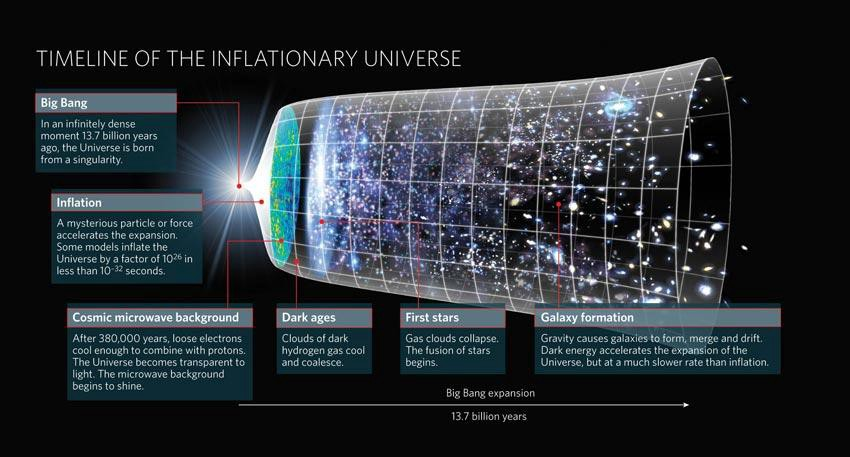
\includegraphics[width=\textwidth]{figure 9.jpeg}
    \caption{A summary of the evolution of the universe}
    \label{fig:final}
\end{figure}

\newpage